\documentclass[10pt,a4paper]{article}

\usepackage[UTF8,fontset = windows]{ctex}

\setCJKmainfont[BoldFont=黑体,ItalicFont=楷体]{等线}

\usepackage{amssymb,amsmath,amsfonts,amsthm,mathrsfs,dsfont,graphicx}

\usepackage{ifthen,indentfirst,enumerate,color,titletoc}

\usepackage{tikz}

\usepackage{multicol}

\usepackage{makecell}

\usepackage{longtable}

\usetikzlibrary{arrows,calc,intersections,patterns,decorations.pathreplacing,3d,angles}

\usepackage[bf,small,indentafter,pagestyles]{titlesec}

\usepackage[top=1in, bottom=1in,left=0.8in,right=0.8in]{geometry}

\renewcommand{\baselinestretch}{1.65}

\newtheorem{defi}{定义~}

\newtheorem{eg}{例~}

\newtheorem{ex}{~}

\newtheorem{rem}{注~}

\newtheorem{thm}{定理~}

\newtheorem{coro}{推论~}

\newtheorem{axiom}{公理~}

\newtheorem{prop}{性质~}

\newcommand{\blank}[1]{\underline{\hbox to #1pt{}}}

\newcommand{\bracket}[1]{(\hbox to #1pt{})}

\newcommand{\onech}[4]{\par\begin{tabular}{p{.9\textwidth}}

A.~#1\\

B.~#2\\

C.~#3\\

D.~#4

\end{tabular}}

\newcommand{\twoch}[4]{\par\begin{tabular}{p{.46\textwidth}p{.46\textwidth}}

A.~#1& B.~#2\\

C.~#3& D.~#4

\end{tabular}}

\newcommand{\vartwoch}[4]{\par\begin{tabular}{p{.46\textwidth}p{.46\textwidth}}

(1)~#1& (2)~#2\\

(3)~#3& (4)~#4

\end{tabular}}

\newcommand{\fourch}[4]{\par\begin{tabular}{p{.23\textwidth}p{.23\textwidth}p{.23\textwidth}p{.23\textwidth}}

A.~#1 &B.~#2& C.~#3& D.~#4

\end{tabular}}

\newcommand{\varfourch}[4]{\par\begin{tabular}{p{.23\textwidth}p{.23\textwidth}p{.23\textwidth}p{.23\textwidth}}

(1)~#1 &(2)~#2& (3)~#3& (4)~#4

\end{tabular}}

\begin{document}

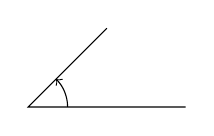
\begin{tikzpicture}\draw (2,0) coordinate (A) -- (0,0) coordinate (B)
-- (1,1) coordinate (C)
pic [draw, ->] {angle};
\end{tikzpicture}

\begin{enumerate}[1.]

\item 从$1,2,3,4,5$中任取两个不同的数, 记``取到的两个数之和为偶数''为事件$A$, ``取到的两个数都大于$2$''为事件$B$, 则$P(A|B)=$\blank{50}.

\item 若$P(A)=0.4$, $P(B)=0.6$, $P(B|A)=0.75$, 则$P(A|B)=$\blank{50}.


\item 甲袋中有$3$个白球和$2$个红球, 乙袋中有$2$个白球和$3$个红球, 丙袋中有$4$个白球和$4$个红球. 先随机取一个袋子, 再从该袋中先后随机取$2$个球.则第一次取出的球是红球的概率为\blank{50}; 在第一次取出的球是红球的条件下, 第二次取出的球是白球的概率为\blank{50}; 第一次取出的球是红球, 且第二次取出的球是白球的概率为\blank{50}.



\item 假设交通事故有$0.6$的概率是因为超速引起的, 则在$8$次交通事故中恰有$6$次是因为超速引起的概率为\blank{50}.


\item 对飞机进行射击, 按照受损伤影响的不同, 飞机的机身可分为两个部分. 要击落飞机, 必须在第一部分命中一次或在第二部分命中两次. 设炮弹击中飞机时, 命中第一部分的概率是$0.3$, 命中第二部分的概率是$0.7$, 射击进行到击落飞机为止. 则每次射击均命中的情况下, 击落飞机的命中次数的分布列为\blank{50}. 



\item 随机变量$X$的分布列为
\[\begin{pmatrix} 1 & 2 & 3 & 4 & 5 \\ \dfrac 18 & \dfrac 14 & \dfrac 14 & \dfrac 14 & \dfrac 18\end{pmatrix},\]
则其期望$E[x]=$\blank{50}; 方差$D[x]=$\blank{50}.

\item 袋中有形状、大小完全相同的$3$个球, 编号分别为$1,2,3$. 从袋中取出$2$个球, 以$X$表示取出的$2$个球中的最大号码, 以$Y$表示取出的$2$个球中的最小号码. 则$E[(X+Y)(X-Y)]=$\blank{50}.

\item 生产方发出了一批产品, 产品共$50$箱, 其中误混了$2$箱不合格产品. 采购方接收该批产品的标准是: 从该批产品中任取$5$箱产品进行检测, 若至多有$1$箱不合格产品, 则接收该批产品. 问: 该批产品被接收的概率是多少? 


\item 飞机的几个发动机彼此独立工作, 测试表明某厂生产的每台发动机出现故障的概率均为$0.004$. 假设飞机正常飞行的条件是至少有一半的发动机能正常工作. 通过建模求解并回答: 一架搭载四台该厂生产的发动机的飞机与一台搭载两台该厂生产的发动机的飞机哪个更安全?


\item 设随机变量$X$的取值在集合$\{0,1,2\}$中.\\
(1) 若$P(X=1)=\dfrac 12$, 求期望$E[X]$的最大可能值$M$与$E[X]$的最小可能值$m$之差;\\
(2) 猜测方差$D[X]$的最大可能值, 并证明你的猜测.

\end{enumerate}

\end{document}